%%%%%%%%%%%%%%%%%%%%%%%%%%%%%%%%%%%%%%%%%%%%%%%%%%%%%%%%%%%%%%%%%%%%
%%%%%%%%%%%%%%%%%%%%%%%%%%%%%%%%%%%%%%%%%%%%%%%%%%%%%%%%%%%%%%%%%%%%
%%                                                                %%
%% Esimerkki opinnäytteen tekemisestä LaTeX:lla                   %%
%% Alkuperäinen versio Luis Costa,  muutokset Perttu Puska        %%
%% Ruotsinkielen tuki lisätty 15092014                            %%
%%                                                                %%
%% Tähän esimerkkiin kuuluu tiedostot                             %%
%%         opinnaytepohja.tex (versio 2.01)                       %%
%%         thesistemplate.tex (versio 2.01) (for text inEnglish)  %%
%%         aaltothesis.cls (versio 2.01)                          %%
%%         kuva1.eps                                              %%
%%         kuva2.eps                                              %%
%%         kuva1.pdf                                              %%
%%         kuva2.pdf                                              %%
%%                                                                %%
%%                                                                %%
%% Kääntäminen joko                                               %%
%% latex:                                                         %%
%%             $ latex opinnaytepohja                             %%
%%             $ latex opinnaytepohja                             %%
%%                                                                %%
%%   Tuloksena on tiedosto opinnayte.dvi, joka                    %%
%%   muutetaan ps-muotoon seuraavasti                             %%
%%                                                                %%
%%             $ dvips opinnaytepohja -o                          %%
%%                                                                %%
%%   ja edelleen pdf-muotoon seuraavasti                          %%
%%                                                                %%
%%             $ ps2pdf opinnaytepohja.ps                         %%
%%                                                                %%
%% Tai                                                            %%
%% pdflatex:                                                      %%
%%             $ pdflatex opinnaytepohja                          %%
%%             $ pdflatex opinnaytepohja                          %%
%%                                                                %%
%%   Tuloksena on tiedosto opinnaytepohja.pdf                     %%
%%                                                                %%
%% Selittävät kommentit on tässä esimerkissä varustettu           %%
%% %%-merkeillä ja muutokset, joita käyttäjä voi tehdä,           %%
%% on varustettu %-merkeillä                                      %%
%%                                                                %%
%%%%%%%%%%%%%%%%%%%%%%%%%%%%%%%%%%%%%%%%%%%%%%%%%%%%%%%%%%%%%%%%%%%%
%%%%%%%%%%%%%%%%%%%%%%%%%%%%%%%%%%%%%%%%%%%%%%%%%%%%%%%%%%%%%%%%%%%%

%% Käytä toinen näistä:
%% ensimmäinen, jos käytät pdflatexia, joka kääntää tekstin suoraan 
%% pdf-tiedostoksi (kuvat on oltava jpg- tai pdf-tiedostoina)
%% toinen, jos haluat tuottaa ps-tiedostoa (käytä eps-formaattia kuville,
%% alä käytä ps-muotoisia kuvia!)
%%
\documentclass[finnish,12pt,a4paper,pdftex,elec,utf8]{aaltothesis}
%\documentclass[finnish,12pt,a4paper,dvips]{aaltothesis}

%% Kirjoita y.o. \documentclass optioiksi
%% korkeakoulusi näistä: arts, biz, chem, elec, eng, sci
%% editorisi käyttämä merkkikoodaustapa: utf8, latin1
%%

%% Käytä näitä, jos kirjoitat englanniksi. Katso englanninokset tiedostosta
%% thesistemplate.tex.
%\documentclass[english,12pt,a4paper,pdftex,elec,utf8]{aaltothesis}
%\documentclass[english,12pt,a4paper,dvips]{aaltothesis}

\usepackage{graphicx}

%% Matematiikan fontteja, symboleja ja muotoiluja lisää, näitä tarvitaan usein 
\usepackage{amsfonts,amssymb,amsbsy}

%% Jos et jostain syystä pidä, miten alla oleva hyperref-paketti käyttää
%% fontteja, värejä yms., käytä tämän paketin makroja muuttamaan
%% fonttimäärittelyt. Katso paketin dokumentaatiota. Paketti määrittelee
%% \url-makron, joten ota paketti käyttöön, jos et käytä hyperref-pakettia.
%%
%\usepackage{url}

%% Saat pdf-tiedoston viittaukset ja linkit kuntoon seuraavalla paketilla.
%% Paketti toimii erityisen hyvin pdflatexin kanssa. 
%%
\usepackage{hyperref}
\hypersetup{pdfpagemode=UseNone, pdfstartview=FitH,
  colorlinks=true,urlcolor=red,linkcolor=blue,citecolor=black,
  pdftitle={Default Title, Modify},pdfauthor={Your Name},
  pdfkeywords={Modify keywords}}


%% Kaikki mikä paperille tulostuu, on tämän jälkeen
\begin{document}

%% Korjaa vastaamaan korkeakouluasi, jos automaattisesti asetettu nimi on 
%% virheellinen 
%%
%% Change the school field to specify your school if the automatically 
%% set name is wrong
% \university{aalto-yliopisto}
% \school{Sähkötekniikan korkeakoulu}

%% Vain kandityölle: Korjaa seuraavat vastaamaan koulutusohjelmaasi
%%
\degreeprogram{Elektroniikka ja sähkötekniikka}
%%

%% VAIN DI/M.Sc.- JA LISENSIAATINTYÖLLE: valitse laitos, 
%% professuuri ja sen professuurikoodi. 
%%
\department{Radiotieteen ja -tekniikan laitos}
\professorship{Piiriteoria}
%%

%% Valitse yksi näistä kolmesta
%%
%\univdegree{BSc}
\univdegree{MSc}
%\univdegree{Lic}

%% Oma nimi
%%
\author{Teemu Teekkari}

%% Opinnäytteen otsikko tulee tähän ja uudelleen englannin- tai 
%% ruostinkielisen abstraktin yhteydessä. Älä tavuta otsikkoa ja
%% vältä liian pitkää otsikkotekstiä. Jos latex ryhmittelee otsikon
%% huonosti, voit joutua pakottamaan rivinvaihdon \\ kontrollimerkillä.
%% Muista että otsikkoja ei tavuteta! 
%% Jos otsikossa on ja-sana, se ei jää rivin viimeiseksi sanaksi 
%% vaan aloittaa uuden rivin.
%% 
\thesistitle{Opinnäyteohje}

\place{Espoo}

%% Kandidaatintyön päivämäärä on sen esityspäivämäärä! 
%% 
\date{16.1.2015}

%% Kandidaattiseminaarin vastuuopettaja tai diplomityön valvoja.
%% Huomaa tittelissä "\" -merkki pisteen jälkeen, ennen välilyöntiä ja
%% seuraavaa merkkijonoa. 
%% Näin tehdään, koska kyseessä ei ole lauseen loppu, jonka jälkeen tulee 
%% hieman pidempi väli vaan halutaan tavallinen väli.
%%
\supervisor{Prof.\ Pirjo Professori} %{Prof.\ Pirjo Professori}

%% Kandidaatintyön ohjaaja(t) tai diplomityön ohjaaja(t). Ohjaajia saa
%% olla korkeintaan kaksi.
%% 
%\advisor{Prof.\ Pirjo Professori}
\advisor{TkT Olli Ohjaaja}
%\advisor{DI Tina Tutkija}

%% Aaltologo: syntaksi:
%% \uselogo{aaltoRed|aaltoBlue|aaltoYellow|aaltoGray|aaltoGrayScale}{?|!|''}
%% Logon kieli on sama kuin dokumentin kieli
%%
\uselogo{aaltoRed}{''}

%% Tehdään kansilehti
%%
\makecoverpage


%% Suomenkielinen tiivistelmä
%% Kaikki tiivistelmässä tarvittava tieto (nimesi, työnnimi, jne.) käytetään
%% niin kuin se on yllä määritelty.
%% Tiivistelmän avainsanat
%%
\keywords{Avainsanoiksi valitaan kirjoituksen sisältöä keskeisesti kuvaavia
käsitteitä}
%% Tiivistelmän tekstiosa
\begin{abstractpage}[finnish]
  Tiivistelmässä on lyhyt selvitys (noin 100 sanaa)
  kirjoituksen tärkeimmästä sisällöstä: mitä ja miten on tutkittu,
  sekä mitä tuloksia on saatu. 
  Tiivistelmässä on lyhyt selvitys (noin 100 sanaa)
  kirjoituksen tärkeimmästä sisällöstä: mitä ja miten on tutkittu,
  sekä mitä tuloksia on saatu. 

  Tiivistelmässä on lyhyt selvitys (noin 100 sanaa)
  kirjoituksen tärkeimmästä sisällöstä: mitä ja miten on tutkittu,
  sekä mitä tuloksia on saatu. 
  Tiivistelmässä on lyhyt selvitys (noin 100 sanaa)
  kirjoituksen tärkeimmästä sisällöstä: mitä ja miten on tutkittu,
  sekä mitä tuloksia on saatu. 
  Tiivistelmässä on lyhyt selvitys (noin 100 sanaa)
  kirjoituksen tärkeimmästä sisällöstä: mitä ja miten on tutkittu,
  sekä mitä tuloksia on saatu. 
\end{abstractpage}

%% Pakotetaan uusi sivu varmuuden vuoksi, jotta 
%% mahdollinen suomenkielinen ja englanninkielinen tiivistelmä
%% eivät tule vahingossakaan samalle sivulle
%%
\newpage
%
%% Opinnäytteen ostikko englanniksi. Poista, jos et tarvitse sitä.
\thesistitle{Thesis template}
%\supervisor{Prof.\ Pirjo Professori}
\advisor{D.Sc.\ (Tech.) Olli Ohjaaja}
%\advisor{M.Sc.\ Polli Pohjaaja}
\degreeprogram{Electronics and electrical engineering}
\department{Department of Radio Science and Technology}
\professorship{Circuit theory}
%% Abstract keywords
\keywords{Resistor, Resistance,\\ Temperature}
%% Abstract text
\begin{abstractpage}[english]
Your abstract in English. Try to keep the abstract short, approximately 
 100 words should be enough. Abstract explains your research topic, 
 the methods you have used, and the results you obtained.  
\end{abstractpage}

%% Force new page so that the Swedish abstract starts from a new page
\newpage
%
%% Ruotsinkiellinen tiivitelmä. Poista, jos et tarvitse sitä.
%% 
%% Opinnäytteen ostikko ruotsiksi.
\thesistitle{Arbetets titel}
%\supervisor{Prof.\ Pirjo Professori}
\advisor{TkD\ Olli Ohjaaja} %
%\advisor{M.Sc.\ Tina Tutkija}
\degreeprogram{Elektronik och elektroteknik}
\department{Institutionen för radiovetenskap och -teknik}%
\professorship{Kretsteori}  %
%% Abstract keywords
\keywords{Nyckelord p\aa{} svenska,\\ Temperatur}
%% Abstract text
\begin{abstractpage}[swedish]
 Sammandrag p\aa{} svenska.
 Try to keep the abstract short, approximately 
 100 words should be enough. Abstract explains your research topic, 
 the methods you have used, and the results you obtained.  
\end{abstractpage}

%% Note that if you are writting your master's thesis in English, place
%% the English abstract first followed by the possible Finnish abstract

%% Esipuhe 
%%
\mysection{Esipuhe}

Haluan kiittää Professori Pirjo 
Professoria ja ohjaajaani Olli Ohjaajaa hyvästä ja 
huonosta ohjauksesta.\\

\vspace{5cm}
Otaniemi, 16.1.2015

\vspace{5mm}
{\hfill Teemu T.\ A.\ Teekkari \hspace{1cm}}

%% Pakotetaan varmuuden vuoksi esipuheen jälkeinen osa
%% alkamaan uudelta sivulta
\newpage


%% Sisällysluettelo
\thesistableofcontents


%% Symbolit ja lyhenteet
\mysection{Symbolit ja lyhenteet}

\subsection*{Symbolit}

\begin{tabular}{ll}
$\mathbf{B}$  & magneettivuon tiheys  \\
$c$              & valon nopeus tyhjössä $\approx 3\times10^8$ [m/s]\\
$\omega_{\mathrm{D}}$    & Debye-taajuus \\
$\omega_{\mathrm{latt}}$ & hilan keskimääräinen fononitaajuus \\
$\uparrow$       & elektronin spinin suunta ylöspäin\\
$\downarrow$     & elektronin spinin suunta alaspäin
\end{tabular}

\subsection*{Operaattorit}

\begin{tabular}{ll}
$\nabla \times \mathbf{A}$              & vektorin $\mathbf{A}$ roottori\\
$\displaystyle\frac{\mbox{d}}{\mbox{d} t}$ & derivaatta muuttujan $t$ suhteen\\
[3mm]
$\displaystyle\frac{\partial}{\partial t}$  & osittaisderivaatta muuttujan $t$ suhteen \\[3mm]
$\sum_i $                       & summa indeksin $i$ yli\\
$\mathbf{A} \cdot \mathbf{B}$    & vektorien $\mathbf{A}$ ja $\mathbf{B}$ pistetulo
\end{tabular}

\subsection*{Lyhenteet}

\begin{tabular}{ll}
AC         & vaihtovirta \\
APLAC      & an object-oriented analog circuit simulator and design tool \\
           & (originally Analysis Program for Linear Active Circuits) \\
BCS        & Bardeen-Cooper-Schrieffer \\ %% tavuviiva - nimien välissä 
DC         & tasavirta \\
TEM        & transverse eletromagnetic
\end{tabular}


%% Sivulaskurin viilausta opinnäytteen vaatimusten mukaan:
%% Aloitetaan sivunumerointi arabialaisilla numeroilla (ja jätetään
%% leipätekstin ensimmäinen sivu tyhjäksi, 
%% ks. alla \thispagestyle{empty}).
%% Pakotetaan lisäksi ensimmäinen varsinainen tekstisivu alkamaan 
%% uudelta sivulta clearpage-komennolla. 
%% clearpage on melkein samanlainen kuin newpage, mutta 
%% flushaa myös LaTeX:n floatit 
%% 
\cleardoublepage
\storeinipagenumber
\pagenumbering{arabic}
\setcounter{page}{1}


%% Leipäteksti alkaa
%%
\section{Johdanto}

%% Ensimmäinen sivu tyhjäksi
%% 
\thispagestyle{empty}

Tämän tekstin lähteenä oleva tiedosto on opinnäytteen
pohja, jota voi käyttää kandidaatintyössä, diplomityössä ja
lisensiaatintyössä. Tekstin 
lähteenä oleva tiedosto on kirjoitettu  \LaTeX-tiedoston rakenteen
opiskelemista ajatellen. Tiedoston kommentit sisältävät
tietoa, joka on hyödyllistä opinnäytettä kirjoitettaessa. 

%% Esimerkki luettelosta. Lyhyt ajatusviiva on käytössä
%% luettelossa, ja se on pituudeltaan
%% en dash. Merkitään latex-koodissa --. 
Johdanto selvittää samat asiat kuin tiivistelmä, mutta
laveammin. Johdannossa kerrotaan yleensä seuraavat asiat

\begin{itemize}
\item[--]Tutkimuksen taustaa ja tutkimusaiheen yleisluonteinen esittely
\item[--]Tutkimuksen tavoitteet
\item[--]Pääkysymys ja osaongelmat
\item[--]Tutkimuksen rajaus ja keskeiset käsitteet.
\end{itemize}

Lyhyiden opinnäytteiden johdannot ovat yleensä liian pitkiä, joten
johdannon paisuttamista on vältettävä. Diplomityöhön sopii johdanto,
joka on 2--4 sivua. %% tässä on myös lyhyt ajatusviiva l. en dash.
Kandidaatintyön johdannon on oltava diplomityön
johdantoa lyhyempi. Sopivasti tiivistetty johdanto ei kaipaa alaotsikoita.


%% Opinnäytteessä jokainen osa alkaa uudelta sivulta, joten \clearpage
%%
\clearpage

\section{Aikaisempi tutkimus}
% \section{Background}

Tässä osassa selvitetään, mitä tutkimuksen kohteena olevasta
aiheesta tiedetään entuudestaan. Selvityksen tulee kattaa
tasapainoisesti koko tutkimuskenttä. 

Kun opinnäytetyötä kirjoitetaan, on noudatettava 
ohjeita, jotka koskevat opinnäytteen rakennetta,
käytäntöjä, muotoseikkoja sekä ulkoasua. Esitellään näitä
ohjeita tarkemmin.

%% Osan hienojaottelua alaosiin, eikä välttämättä edes tarpeen,
%% tässä vain esimerkkinä. Käytä harkintasi mukaan
%% osan jaottelua, joskus alaotsikot selventävät asioita ja
%% joskus vain sirpaloittavat tarpeettomasti tekstiä.
%%  Jaottelu menee seuraavasti:
%% \section{osan otsikko} 
%% \subsection{alaotsikko}
%% \subsubsection{ala-alaotsikko}
%% Tätä pitemälle ei pidä jaotella. 
%%
%% Three levels of hierarchy in sectioning should be enough

\subsection*{Rakenne}

Opinnäytteen rakenteen tulee olla hyvän tieteellisen
kirjoittamisen käytännön mukainen ja sisältää vähintään seuraavat
osat:

\begin{enumerate}
\item Nimiölehti
\item Tiivistelmä
\item Sisällysluettelo
\item Symboli- ja lyhenneluettelo
\item \label{a} Johdanto
%% Tässä alla on esimerkki lainausmerkkien käytöstä. Suomalaisen tekstin
%% lainausmerkit eivät mene oikein latexissa (tai monissa muissakaan
%% julkaisujärjestelmissä) kun käytetään
%% "-merkkiä, koska latex käyttää amerikkalaista lainausmerkkien
%% tulostustapaa. Vaihtoehtona voi käyttää kulmalainausmerkkejä, jotka
%% myös tulostuvat oikein.
\item  Aikaisempi tutkimus. Työn luonteen niin vaatiessa otsikko voi olla myös
        >>Teoreettinen tausta>>  tai näiden otsikoiden yhdistelmä.
\item Tutkimusaineisto ja -menetelmät %% yhdysmerkki - eli tavuviiva. 
\item Tulokset
\item \label{o} Tarkastelu. Työn luonteen niin vaatiessa otsikko voi
      olla myös >>Johtopäätökset>> tai >>Yhteenveto>> 
      tai edellä mainittujen otsikoiden yhdistelmä.
\item Lähteet
\item Liitteet.
\end{enumerate}

Tiivistelmän ja symboli- sekä lyhenneluetteloiden 
väliin voi sijoittaa halutessaan esipuheen.  

Työn osat \ref{a}-\ref{o} muodostavat \textit{tekstiosan.}  Työn
yksittäisiä osia voidaan jakaa alaotsikoilla alaosiin, joita ei ole
yllä esitetty. Alaotsikoiden käyttäminen selventää parhaimmillaan
tekstiä, ja pahimmillaan sirpaloittaa sitä.  Sirpaloitumista voi estää
huolehtimalla siitä, että samalla sivulla ei esiinny useampaa
alaotsikkoa.  Tekstin jäsentelyssä on yleensä ongelmia, jos osassa on
vain yksi alaosa, tai kirjoittaja joutuu käyttämään useampaa kuin
kahta tasoa (osa ja alaosat): alaosien alaosat ovat harvoin tarpeen.
\subsection*{Sivut ja kirjaintyypit}

Opinnäytteen tulee olla kirjoitettu koneella tai
tekstinkäsittelyohjelmalla yksipuolisesti A4-kokoiselle paperille.
Kandidaatintyön tekstiosan sopiva pituus on noin 15--20 sivua ja
diplomityön noin 60 sivua. Työtä ei ole syytä tarpeettomasti pidentää.

Opinnäytteen tekstiosan kirjaintyypin tulee olla antiikva eli
%% esimerkki pakkotavutuksesta; "serif-tyyppinen" on tavutuksen kannalta
%% hankala, joten pakkotavutetaan se. 
serif\--tyyp\-pi\-nen ja lisäksi kursivoimaton, lihavoimaton sekä kooltaan 12
pistettä (kuten tässä esityksessä). Groteskeja eli \textsf{Sans
  serif}-tyyppisiä kirjaintyyppejä (kuten Helvetica tai Arial) ei saa
käyttää varsinaisessa tekstissä, mutta otsikoissa näitä voidaan
käyttää.  Otsikoissa voidaan käyttää kooltaan edellä mainittua
suurempaa kirjaintyyppiä sekä tyylikeinoja, kuten lihavointia tai
kursivointia.  Tekstissä samantasoisten otsikoiden on kuitenkin oltava
tyyliltään ja kirjainlajeiltaan yhteneväisiä.
%% Esimerkki taulukosta
\begin{table}[htb]
%% Taulukon teksti
\caption{Taulukoissa ja kuvissa kirjaintyypin voi valita
tarkoituksenmukaisesti, mutta kuva- ja taulukkoteksteissä tulee
käyttää samaa kirjaintyyppiä kuin varsinaisessa tekstissä. 
Huomaa taulukon numeroinnin sijoittuminen taulukon yläpuolelle. \label{taulukko1}}
\begin{center}
\fbox{
\begin{tabular}{c|l|r}
\textbf{A} & 1 & $e^{j \omega t}$ \\ \hline
\textsf{B} & 2 & ${\mathfrak R}(c)$ \\ \hline
\texttt{C} & 3 & $ a \in \mathbb{A}$  
\end{tabular}
}
\end{center}
\end{table}

Opinnäytteen vasen marginaali (sidonnan puoli) on
35~mm % tässä ~ muodostaa ns. yhdistävän välilyönnin
ja oikea 25~mm. Ylämarginaali on 25~mm. Leipätekstin korkeus on
enimmillään 230mm. Tämän opinnäytepohjan marginaalien pitäisi olla
paperille tulostettuna oikein, mutta tulostimesta ja paperista
riippuen voi esiintyä yhden tai kahden millimetrin suuruisia eroja.
%% Jos käännät tämän tekstin pdflatex-komennolla ja tulostat sen katselu-
%% ohjelmasta, toteat todennäköisesti em. mittojen poikkeavan enemmän
%% kuin 1-2 mm. 
%% Tämä on seurausta pdf-tiedoston erilaisesta kirjaintyyppimäärityksestä.
%% Korkeatasoista painotyötä varten käytä vain latex-komentoa ja 
%% tulosta postscript-muotoon käännetystä tiedostosta. 
\subsection*{Asemointi}

%% Muutos vanhaan ohjeeseen verrattuna: aikaisemmassa ohjeessa
%% kehotettiin käyttämään vasensuora-asettelua, mutta tässä
%% ohjeessa ollaan luovuttu tuosta vaatimuksesta ja siirrytty
%% huoliteltumpaan, painotuotteenomaisempaan suuntaan.  
Tekstiosan tekstissä käytetään kappaleiden erottamiseen sisennystä,
mutta ensimmäistä otsikon, väliotsikon tai muun katkon jälkeistä
kappaletta ei sisennetä. Jos kuva tai muu katko tulee kappaleiden
väliin, suositellaan katkon jälkeisen kappaleen sisentämistä.

Mikäli oikea reuna halutaan tasata, tulee käyttää tavutusta ja lisäksi
tarkistaa, ettei tekstiin jää lukemista häiritseviä pitkiä sanavälejä. Jos
käytät opinnäytteen tekemisessä \LaTeX-järjestelmää, 
tämä asia hoituu automaattisest.

Opinnäytteen riviväli on 1, mikä on myös tämän opinnäytepohjan käytäntö. 
Kappaleiden tulee yleensä olla ainakin kolmen rivin pituisia, mutta
myös liian pitkiä kappaleita tulee välttää.  Tässä opinnäytepohjassa
ei tekstin luonteen vuoksi voida täysin toteuttaa kappaleen pituutta koskevia
vaatimuksia.

Yksittäisiä, kappaleen päättäviä tai aloittavia rivejä sivun alussa
tai lopussa on vältettävä koko työssä, myös luetteloissa ja
liitteissä.

\subsection*{Numerointi}

Opinnäytteen jokainen osa alkaa uudelta sivulta. Alaosa aloittaa uuden
sivun vain edellisen sivun täytyttyä.

Työn osat numeroidaan siten, että johdanto on ensimmäinen numeroitava
osa. Osien numeroinnissa käytetään arabialaisia numeroita.

Nimiölehti, tiivistelmä, esipuhe, sisällysluettelo ja symboli- ja
lyhenneluettelo numeroidaan esipuheesta tai tämän puuttuessa 
ensimmäiseltä luettelosivulta alkaen roomalaisin numeroin.

Sivunumerointi alkaa toiselta varsinaiselta tekstisivulta, ja 
sivunumeroinnissa käytetään arabialaisia numeroita.

Lähdeluettelo alkaa uudelta sivulta. Lähdeluettelon sivunumerointi 
jatkuu viimeisestä tekstisivusta.

Jokainen liite alkaa uudelta sivulta. Liitteiden sivunumerointi
jatkuu viimeisestä lähdeluettelon sivusta.

Sivunumero sijoitetaan sivun yläreunaan.

Matemaattiset kaavat numeroidaan arabialaisin
numeroin. Kaavanumerointi ei saa katketa osien välissä (eikä niin
tapahdukaan, jos käytät tätä opinnäytepohjaa). Kaikkia kaavoja ei tarvitse
numeroida, vaan kirjoittaja voi käyttää harkintaa numeroinnin
tarpeellisuudessa.  Liitteissä olevat kaavat numeroidaan siten, että
liitteen ajatellaan muodostavan numeroinnin kannalta itsenäisen ja
yhtenäisen kokonaisuuden. Kaavan numero sijoitetaan oikealle puolelle
alla olevan esimerkin mukaisesti
\begin{equation}
D(xy) = (Dx)y + x(Dy),  \hspace{3em} x,y \in \mathbb{A}.
\end{equation}
%% Kaavojen jälkeen ei yleensä laiteta sisennystä. 
Kaikki kuvat ja taulukot numeroidaan erillisen juoksevan numeroinnin
mukaisesti kuten taulukosta \ref{taulukko1} ja kuvasta \ref{kuva1} käy
ilmi.  Liitteissä olevat kuvat ja taulukot numeroidaan siten, että
liitteen ajatellaan muodostavan numeroinnin kannalta itsenäisen ja
yhtenäisen kokonaisuuden. Liitteissä \ref{LiiteA} ja \ref{LiiteB} on
esimerkkejä kaavojen (kaavat \ref{liitekaava1}--\ref{liitekaava2} tai
kaavat \ref{liitekaava3}--\ref{liitekaava4}), kuvien (kuva
\ref{liitekuva}) ja taulukoiden (taulukko \ref{liitetaulukko})
numeroimisesta.  Liitteet numeroidaan suuraakkosin (esimerkiksi Liite
A, Liite B tai pelkästään A, B).
%% Tässä esimerkki kuva1.pdf -nimisen tiedoston tuomisesta kuvaksi.
%% Komento \inclugraphics[parametrit]{argumentti} tuo kuvan.
%% Komento \centering pakottaa kuvan keskelle. 
%% Komento \caption luo kuvatekstin ja sen numeroinnin
%% Parametrit htb pakottavat kuvan suunnilleen siihen 
%% kohtaan, missä se esiintyy tekstin lähdekoodissa
\begin{figure}[htb]
\centering 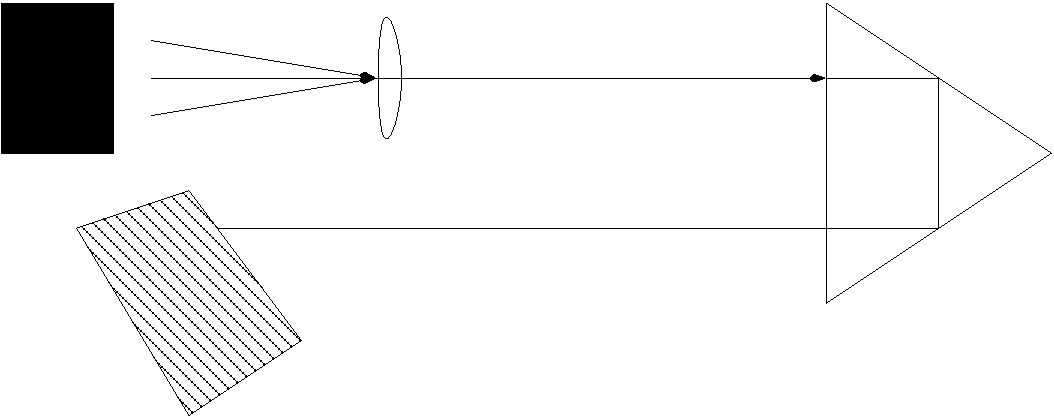
\includegraphics[height=5cm]{kuva1}
\caption{Tämä on esimerkki numeroidusta kuvatekstistä. \label{kuva1}}
\end{figure}

\subsection*{Lähdeviittausten käyttö} 

Lähdeviittaukset tulee tehdä huolellisesti ja johdonmukaisesti
numeroviitejärjestelmän mukaisesti. Numeroviitteet järjestetään
lähdeluetteloon viittausjärjestykseen, mutta jos lähdeluettelo
on hyvin laaja (useita sivuja), järjestetään viitteet pääsanan 
mukaiseen aakkosjärjestykseen. Alaviitejärjestelmää
\footnote{Myöskään alaviitteenä olevia kommentteja \underline{ei} suositella
käytettäviksi.} ei käytetä. 

Viitteen sijoittelussa noudatetaan seuraavia sääntöjä:
Jos viite kohdistuu vain yhteen virkkeeseen tai virkkeen 
osaan, viite \cite{Kauranen} sijoitetaan virkkeen sisään ennen virkettä
päättävää pistettä. Jos taas viite koskee tekstin useampaa
virkettä tai kokonaista kappaletta, sijoitetaan viite kappaleen loppuun 
pisteen jälkeen. \cite{Kauranen} 

\subsection*{Lähdeluettelo} 

Lähdeluettelossa esiintyy tavallisesti seuraavassa esitettäviä
lähteitä, joista on numeroviitejärjestelmässä ilmoitettava
asianomaisessa kohdassa vaaditut tiedot.

%% Esimerkki korostamisesta. Lihavoinnin sijasta on tyylikkäämpää
%% ja luettavampaa käyttää kursiivia.
\textit{Kirjasta} ilmoitetaan seuraavat tiedot:

\begin{itemize}
\item[--]tekijät 
\item[--]julkaisun nimi
\item[--]painos, jos useita
\item[--]kustannuspaikka
\item[--]julkaisija tai kustantaja
\item[--]julkaisuaika
\item[--]mahdollinen sarjamerkintö. 
\end{itemize}

Viitteet \cite{Kauranen}--\cite{Koblitz} ovat esimerkkejä kirjan
esittämisestä lähdeluettelossa. Viite \cite[s.\ 83--124]{Koblitz} on
esimerkki lähdeluettelossa esiintyvän kirjan tiettyjen sivujen
esittämisestä tekstissä.

\textit{Artikkelista} kausijulkaisussa ilmoitetaan seuraavat tiedot:

\begin{itemize}

\item[--]tekijät
\item[--]artikkelin nimi
\item[--]kausijulkaisun nimi
\item[--]julkaisuvuosi
\item[--]kausijulkaisun volyymi tai ilmestymisvuosi
\item[--]kausijulkaisun numero
\item[--]sivut, joilla artikkeli on.
\end{itemize}

Viitteet \cite{bcs}--\cite{Deschamps} ovat esimerkkejä artikkelin
esittämisestä lähdeluettelossa.

\textit{Kokoomateoksen luvusta tai osasta} ilmoitetaan seuraavat tiedot:

\begin{itemize}
\item[--]luvun tai osan tekijät
\item[--]luvun tai osan nimi
\item[--]maininta >>Teoksessa>>
\item[--]koko teoksen toimittajat sekä maininta >>(toim.)>>
\item[--]koko teoksen tai konferenssin nimi
\item[--]konferenssiesitelmän kyseessä ollessa sen pitopaikka ja -aika
\item[--]painos, jos useita
\item[--]kustannuspaikka
\item[--]julkaisija tai kustantaja, jos aihetta tämän ilmoittamiseen on
\item[--]julkaisuaika
\item[--]sivut, joilla luku tai osa on 
\item[--]mahdollinen sarjamerkintä.
\end{itemize}

Viitteet \cite{Sihvola}--\cite{Lindblom} ovat esimerkkejä
kokoomateoksen luvun tai osan esittämisestä lähdeluettelossa. 

\textit{Opinnäytetyöstä} ilmoitetaan seuraavat tiedot:

\begin{itemize}
\item[--]tekijä
\item[--]työn nimi
\item[--]opinnäytetyön tyyppi
\item[--]oppilaitoksen nimi
\item[--]osaston, laitoksen tai ohjelman nimi
\item[--]oppilaitoksen sijaintipaikka
\item[--]vuosiluku.
\end{itemize}

Viitteet \cite{Miinusmaa}--\cite{Lonnqvist} ovat esimerkkejä
opinnäytteen esittämisestä lähdeluettelossa. 

\textit{Standardista} ilmoitetaan seuraavat tiedot:

\begin{itemize}
\item[--]standardin tunnus ja numero
\item[--]standardin nimi
\item[--]painos, mikäli ei ole ensimmäinen
\item[--]julkaisupaikka
\item[--]julkaisija
\item[--]julkaisuvuosi
\item[--]sivumäärä.
\end{itemize}
Viite \cite{sfs} on esimerkki standardin esittämisestä opinnäytteen
lähdeluettelossa. 

\textit{Haastattelusta} ilmoitetaan seuraavat tiedot:

\begin{itemize}
\item[--]haastatellun henkilön nimi
\item[--]haastatellun henkilön arvo tai asema
\item[--]haastatellun henkilön edustama organisaatio
\item[--]organisaation osoite
\item[--]maininta siitä, että kyseessä on haastattelu ja haastattelun
päivämäärä. 
\end{itemize}

Viite \cite{haastattelu} on esimerkki 
haastattelun esittämisestä lähdeluettelossa.

Osa sähköisessä muodossa olevista artikkeleista on saatavissa myös
painettuina. \textit{Vain verkosta saatavissa olevasta artikkelista} esitetään
seuraavat tiedot:

\begin{itemize}
\item[--]tekijät
\item[--]artikkelin nimi
\item[--]kausijulkaisun nimi
\item[--]viestintyyppi
\item[--]laitos tai volyymi
\item[--]kausijulkaisun yksittäistä osaa koskeva merkintä tai numero
\item[--]julkaisuvuosi tai maininta >>Päivitetty>> ja päivitysaika
\item[--]maininta >>Viitattu>> ja viittaamisen ajankohta 
\item[--]maininta >>Saatavissa>> ja URL tai 
        maininta >>DOI>> ja DOI-numero (DOI=Digital Object Identifier).
\end{itemize}

Viitteet \cite{Ribeiro}--\cite{kone} ovat esimerkkejä sähköisessä
muodossa olevan artikkelin esittämisestä opinnäytteen
lähdeluettelossa.  Viitteet \cite{Ribeiro} ja \cite{Stieber} ovat
saatavissa sekä painettuna että verkosta, joten viitteiden esitystapa
mukailee painetun artikkelin viitteen esitystapaa, mutta sen lisäksi
kerrotaan julkaisun olevan verkkolehti ja lehden olevan saatavissa
myös painettuna.  Viite \cite{kone} on saatavissa vain verkosta ja
siitä esitetään yllä vaaditut tiedot.

Valitettavasti sähköisessä muodosssa olevasta artikkelista ei ole aina 
saatavissa lai\-tos-, volyymi- tai numerotietoja.

\textit{Sähköisessä muodossa olevasta opinnäytetyöstä} ilmoitetaan
seuraavat tiedot:
 
\begin{itemize}
\item[--]tekijä
\item[--]työn nimi
\item[--]viestintyyppi
\item[--]opinnäytetyön tyyppi
\item[--]oppilaitoksen nimi
\item[--]osaston, laitoksen tai ohjelman nimi
\item[--]oppilaitoksen sijaintipaikka
\item[--]vuosiluku
\item[--]viittamisen ajankohta
\item[--]maininta >>Saatavissa>> ja URL tai 
        maininta >>DOI>> ja DOI-numero.
\end{itemize}

Viite \cite{Adida} on esimerkki sähköisessä muodossa olevan
opinnäytteen esittämisestä lähdeluettelossa.

Viite \cite{viittaaminen} on esimerkki itsenäisen kirjoituksen sisältävästä
verkkosivusta. Tällainen lähde on rinnastettavissa erillisteokseen.
\textit{Verkkosivusta} esitetään tiedot:

\begin{itemize}
\item[--] tekijät
\item[--] otsikko
\item[--] maininta >>Päivitetty>> ja päivitysaika 
\item[--] maininta >>Viitattu>> ja viittaamisen ajankohta
\item[--] Maininta >>Saatavissa>> ja URL.
\end{itemize}

Joskus verkkosivun kirjoitus on jaettu useammalle sivulle, jolloin
lähdeluetteloon kirjataan vain sellainen verkko-osoite, joka koskee
koko kirjoitusta tai sen etusivua, ellei sitten 
todella tarkoiteta kirjoituksen yksittäistä sivua. 

\subsection*{Muuta huomioitavaa lähdeluettelossa}

%% Muutos vanhoihin ohjeisiin koskien kieltä.
Lähdeluettelossa työn ja julkaisun nimi kirjoitetaan alkuperäisessä
muodossaan. Julkaisijan kotipaikka kirjoitetaan alkukielisessä
muodossaan.

Viittamista koskevassa suomalaisessa standardissa
SFS 5342 \cite{sfs} vaaditaan julkaisuista ilmoitettavaksi myös ISBN- tai
ISSN-numerot, mutta näissä opinnäyteohjeissa ei ISBN- ja 
ISSN-numeroita vaadita. 

\clearpage

\section{Tutkimusaineisto ja -menetelmät}

Tässä osassa kuvataan käytetty tutkimusaineisto ja
tutkimuksen metodologiset valinnat, sekä
kerrotaan tutkimuksen toteutustapa ja käytetyt menetelmät. 

\clearpage

\section{Tulokset}

Tässä osassa esitetään tulokset ja vastataan tutkielman alussa
esitettyihin tutkimuskysymyksiin. Tieteellisen kirjoitelman
arvo mitataan tässä osassa esitettyjen tulosten perusteella. 

%% Huomaa seuraavassa kappaleessa lainausmerkkien ulkopuolella piste, 
%% koska piste ei lopeta lainattua tekstinpätkää.
%% Jos lainattu tekstinpätkä loppuu välimerkkiin, tulee välimerkki
%% lainausmerkkien sisälle: 
%% "Et tu, Brute?" sanoi Caesar kuollessaan.
Tutkimustuloksien merkitystä on aina syytä arvioida ja tarkastella
kriittisesti.  Joskus tarkastelu voi olla tässä osassa, mutta se
voidaan myös jättää viimeiseen osaan, jolloin viimeisen osan nimeksi
tulee >>Tarkastelu>>. Tutkimustulosten merkitystä voi arvioida myös
>>Johtopäätökset>>-otsikon alla viimeisessä osassa. 

Tässä osassa on syytä myös arvioida tutkimustulosten luotettavuutta.
Jos tutkimustulosten merkitystä arvioidaan >>Tarkastelu>>-osassa,
voi luotettavuuden arviointi olla myös siellä. 

\clearpage

\section{Yhteenveto}
%\section{Summary} 

Opinnäytteen tekijä vastaa siitä, että opinnäyte on tässä dokumentissa
ja opinnäytteen tekemistä käsittelevillä luennoilla sekä
harjoituksissa annettujen ohjeiden mukainen muotoseikoiltaan,
rakenteeltaan ja ulkoasultaan.



\clearpage
%% Lähdeluettelo

\thesisbibliography

\begin{thebibliography}{99}

%% Alla pilkun jälkeen on pakotettu oikea väli \<välilyönti>-merkeillä.
\bibitem{Kauranen} Kauranen,\ I., Mustakallio,\ M. ja Palmgren,\ V.
  \textit{Tutkimusraportin kirjoittamisen opas opinnäytetyön
    tekijöille.}  Espoo, Teknillinen korkeakoulu, 2006.

\bibitem{Itkonen} Itkonen,\ M. \textit{Typografian käsikirja.} 3.\
  painos.  Helsinki, RPS-yhtiöt, 2007.

\bibitem{Koblitz} Koblitz,\ N. \textit{A Course in Number Theory and
    Cryptography. Graduate Texts in Mathematics 114.}  2.\ painos. New
  York, Springer, 1994.

%% Kun on useampi nimikirjain, jokaisen nimikirjaimen väliin
%% kuuluu välilyönti. Oikea välin määrä on saatu \<välilyönnillä>
\bibitem{bcs} Bardeen,\ J., Cooper,\ L.\ N. ja Schrieffer,\ J.\ R.
  Theory of Superconductivity. \textit{Physical Review,} 1957, vol.\
  108, nro~5, s.\ 1175--1204.

\bibitem{Deschamps} Deschamps,\ G.\ A. Electromagnetics and
  Differential Forms. \textit{Proceedings of the IEEE,} 1981, vol.\
  69, nro~6, s.\ 676--696.

%% Alla esimerkki englanninkielisen tavuttamisen pakottamisesta.
%% Oletusarvoisesti käytetään suomalaista tavutusta, mutta viitteissä
%% esiintyy usein muunkielisiä lauseita, jotka tulevat siten tavutetuksi
%% suomen kielen sääntöjen mukaan. Tämän voi korjata \foreignlanguage-
%% komennolla, jonka ensimmäinen parametri on vieraan kielen nimi ja toinen 
%% on vieraalla kielellä tavutettava teksti. 
\bibitem{Sihvola} Sihvola,\ A.\ et al.
  \foreignlanguage{english}{Interpretation of measurements of helix 
    and bihelix superchiral structures.}
  Teoksessa: Jacob,\ A.\ F. ja
  Reinert,\ J. (toim.) \textit{Bianisotropics '98 7th International
    Conference on Complex Media.}  Braunschweig, 3.--6.6.1998.
  Braunscweig, Technische Universität Braunschweig, 1998, s.\
  317--320.

%% Alla on suomalainen yhdistelmäsukunimi. Sen nimien välissä 
%% käytetään yhdysmerkkiä l. tavuviivaa, kirjoitetaan -.
\bibitem{Lindblom} Lindblom-Ylänne,\ S. ja Wager,\ M.  Tieteellisten
  opinnäytetöiden ohjaaminen. Teoksessa: Lindblom-Ylänne,\ S. ja
  Nevgi,\ A. (toim.) \textit{Yliopisto- ja korkeakouluopettajan
    käsikirja.}  Helsinki, WSOY, 2004, s.\ 314--325.
 
\bibitem{Miinusmaa} Miinusmaa,\ H. Neliskulmaisen reiän poraamisesta
  kolmikulmaisella poralla. Diplomityö, Teknillinen korkeakoulu,
  konetekniikan osasto, Espoo, 1977.

%% Tässä taas pakotettu englanninkielinen tavutus. 
%% Pedanttinen kirjoittaja pakottaa tietysti jokaiseen englanninkieliseen
%% lauseeseen englannin tavutuksen, mutta tässä esityksessä ei näin ole
%% tehty selvyyden ja lähdekoodin luettavuuden takia. 
\bibitem{Loh} Loh,\ N.\ C. High-Resolution Micromachined
  Interferometric Accelerometer. Master's Thesis, Massachusetts
  Institute of Technology, Cambridge,
  \foreignlanguage{english}{Massachusetts,} 1992.

\bibitem{Lonnqvist} Lönnqvist,\ A.
  \foreignlanguage{english}{Applications of hologram-based compact
    range: antenna radiation pattern, radar cross section, and
    absorber reflectivity measurements.}
  Väitöskirja, Teknillinen korkeakoulu, sähkö- ja tietoliikennetekniikan
  osasto, 2006.

\bibitem{sfs} SFS 5342. Kirjallisuusviitteiden laatiminen. 2.\ painos.
  Helsinki, Suomen standardisoimisliitto, 2004. 20~s.

\bibitem{haastattelu} Palmgren,\ V. Suunnittelija. Teknillinen
  korkeakoulu, kirjasto. Otaniementie 9, 02150 Espoo. Haastattelu
  15.1.2007.

\bibitem{Ribeiro} Ribeiro,\ C.\ B., Ollila,\ E. ja Koivunen,\ V.
  \foreignlanguage{english}{Stochastic Maximum-Likelihood Method for
    MIMO Propagation Parameter Estimation.}
 \textit{IEEE Transactions
    on Signal Processing,} verkkolehti, vol.\ 55, nro~1, s.\ 46--55.
  Viitattu 19.1.2007. Lehti ilmestyy myös painettuna. DOI:
  10.1109/TSP.2006.882057.

\bibitem{Stieber} Stieber,\ T. GnuPG Hacks. \textit{Linux Journal,}
  verkkolehti, 2006, maaliskuu, nro~143. Viitattu 19.1.2007. Lehti
  ilmestyy myös painettuna. Saatavissa:
  \url{http://www.linuxjournal.com/article/8732.}

\bibitem{kone} Pohjois-Koivisto,\ T. Voiko kone tulevaisuudessa arvata
  tahtosi?  \textit{Apropos,} verkkolehti, helmikuu, nro~1, 2005.
  Viitattu 19.1.2007.  Saatavissa:
  \url{http://www.apropos.fi/1-2005/prima.php.}

\bibitem{Adida} Adida,\ B.  Advances in Cryptographic Voting Systems.
  Verkkodokumentti. Ph.D.\ Thesis, Massachusetts Institute of
  Technology, Cambridge, 
  \foreignlanguage{english}{Massachusetts,}
  2006. Viitattu 19.1.2007.  Saatavissa:
  \url{http://crypto.csail.mit.edu/~cis/theses/adida-phd.pdf.}

\bibitem{viittaaminen} Kilpeläinen,\ P. WWW-lähteisiin viittaaminen
  tutkielmatekstissä. Verkkodokumentti. Päivitetty 26.11.2001.
  Viitattu 19.1.2007. Saatavissa:
  \url{http://www.cs.uku.fi/~kilpelai/wwwlahteet.html.}

\end{thebibliography}

%% Liitteet
\clearpage

\thesisappendix

\section{Esimerkki liitteestä\label{LiiteA}}

Liitteet eivät ole opinnäytteen kannalta välttämättömiä ja 
opinnäytteen tekijän on 
kirjoittamaan ryhtyessään hyvä ajatella pärjäävänsä ilman liitteitä.
Kokemattomat kirjoittajat, jotka ovat huolissaan
tekstiosan pituudesta, paisuttavat turhan 
helposti liitteitä pitääkseen tekstiosan pituuden annetuissa rajoissa.
Tällä tavalla ei synny hyvää opinnäytettä.   

Liite on itsenäinen kokonaisuus, vaikka se täydentääkin tekstiosaa.
Liite ei siten ole pelkkä listaus, kuva tai taulukko, vaan 
liitteessä selitetään aina sisällön laatu ja tarkoitus. 

Liitteeseen voi laittaa esimerkiksi listauksia. Alla on 
listausesimerkki tämän liitteen luomisesta. 

%% Verbatim-ympäristö ei muotoile tai tavuta tekstiä. Fontti on monospace.
%% Verbatim-ympäristön sisällä annettuja komentoja ei LaTeX käsittele. 
%% Vasta \end{verbatim}-komennon jälkeen jatketaan käsittelyä.
\begin{verbatim}
	\clearpage
	\appendix
	\addcontentsline{toc}{section}{Liite A}
	\section*{Liite A}
	...
	\thispagestyle{empty}
	...
	tekstiä
	...
	\clearpage
\end{verbatim}

Kaavojen numerointi muodostaa liitteissä oman kokonaisuutensa:
\begin{eqnarray}
d \wedge A  &=& F, \label{liitekaava1}\\
d \wedge F  &=& 0. \label{liitekaava2}
\end{eqnarray}


\clearpage
\section{Toinen esimerkki liitteestä\label{LiiteB}}

%% Liitteiden kaavat, taulukot ja kuvat numeroidaan omana kokonaisuutenaan

Liitteissä voi myös olla kuvia, jotka
eivät sovi leipätekstin joukkoon:
%% Ympäristön figure parametrit htb pakottavat
%% kuvan tähän, eikä LaTeX yritä siirrellä niitä
%% hyväksi katsomaansa paikkaan. 
%% Ympäristöä center voi käyttää \centering-
%% komennon sijaan
%%
\begin{figure}[htb]
\begin{center}
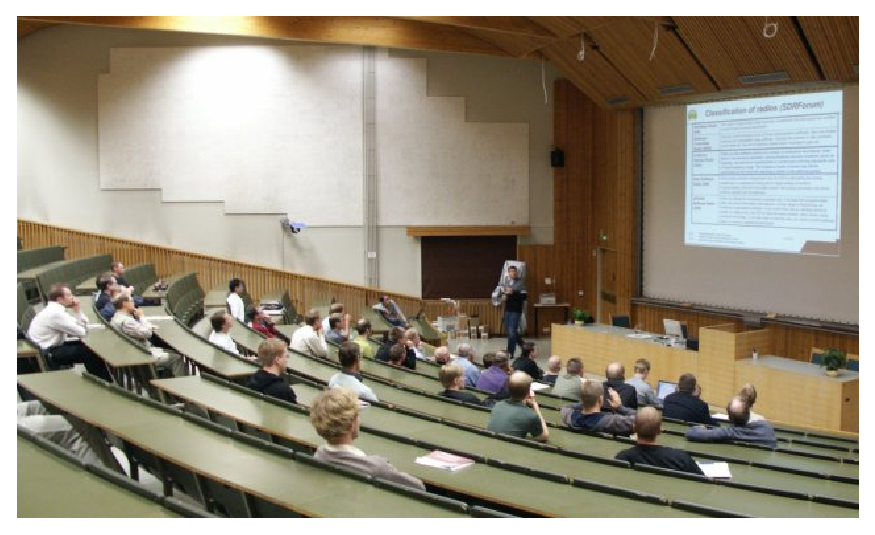
\includegraphics[height=8cm]{kuva2}
\end{center}
\caption{Kuvateksti, jossa on liitteen numerointi}
\label{liitekuva}
\end{figure}
%%
Liitteiden taulukoiden numerointi on kuvien ja kaavojen kaltainen:
\begin{table}[htb]
\caption{Taulukon kuvateksti.}
\label{liitetaulukko}
\begin{center}
\fbox{
\begin{tabular}{lp{0.5\linewidth}}
9.00--9.55  & Käytettävyystestauksen tiedotustilaisuus (osanottajat
ovat saaneet sähköpostitse valmistautumistehtävät, joten tiedotustilaisuus
voidaan pitää lyhyenä).\\
9.55--10.00 & Testausalueelle siirtyminen
\end{tabular}}
\end{center}
\end{table}
Kaavojen numerointi muodostaa liitteissä oman kokonaisuutensa:
\begin{eqnarray}
T_{ik} &=& -p g_{ik} + w u_i u_k + \tau_{ik},  \label{liitekaava3} \\
n_i    &=& n u_i + v_i.                      \label{liitekaava4}
\end{eqnarray}

\end{document}
